\documentclass{article}
\usepackage{graphicx}
\usepackage{float}% Required for inserting images

\title{How do citizens perceive their similarity to one another in terms of demographic characteristics?}
\author{Aryan Goyal}
\date{March 2024}

\begin{document}
\maketitle

\section{Original Study}
I replicate this study: "Titelman, N. (2023). Class, Ethnicity, Age or Education: What Characteristics Determine Citizens' Sense of Political Commonality?. British Journal of Political Science, 53(2), 806-814."

It attempts to compare the relative strength of different social identities in the population from the perspective of how citizens perceive one another politically, rather than from their tendency to vote together.
\\
\\
Existing literature has focused largely on how demographic
characteristics (Ethnicity,  Age) themselves explain vote choice
\\
\\
The author suggests analysing the associations between demographic groups 
and voting does not reveal the relative importance of the corresponding 
social identities to politics
\\
\\
Hence, Titelman hopes to understand which characteristics (Gender, 
ethnicity etc) are more important for people to feel a sense of political 
commonality with others
\\
This paper has no stated hypotheses
\\
\\
Method:
\\
In order to study political commonality, respondents are presented with the profiles of two fellow citizens, including several demographic attributes.
\\
Respondents are asked which of the two they perceive themselves to have more in common with in terms of politics
\begin{figure} [H]
    \centering
    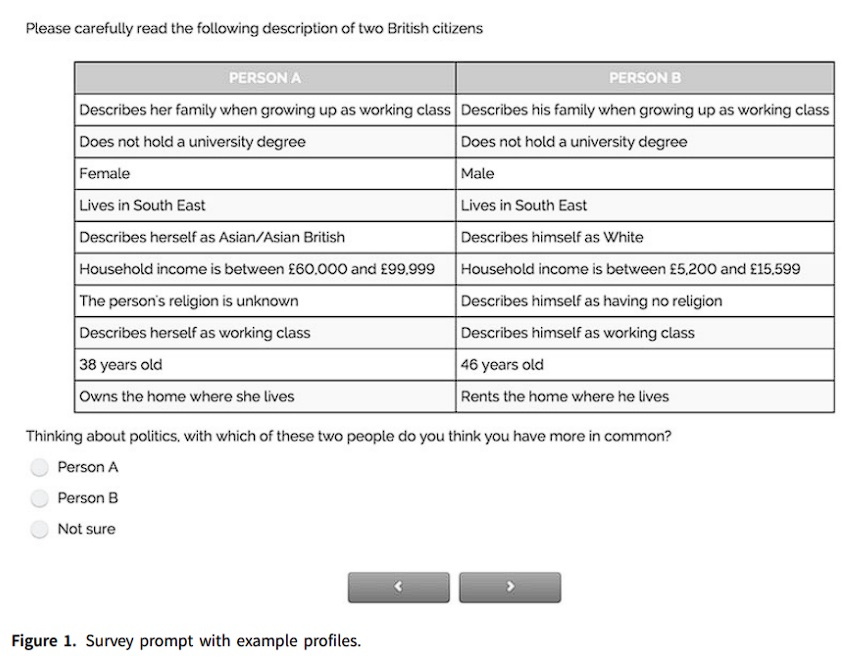
\includegraphics[width=1.3\textwidth]{Figure 1.jpg}
    \caption{Figure 1 from Original Study}
    \label{fig:enter-label}
\end{figure}




\section{Data}

\begin{verbatim}
    load("CleanDataExperiment2")
\end{verbatim}
\\
Input variable:
\\
(Characteristic) of respondent matches with the (Characteristic) 
in profile, coded as:
\\
(Characteristic) matches in profile A: 1
\\
(Characteristic) matches in both/neither: 0
\\
(Characteristic) matches in profile B: -1
\\
\\
The (characteristics) included in the study were: Gender, Age, Religion, Region, Home status, Education, Annual household income, Subjective class and Subjective family class
\\
\\
Outcome variable:
\\
Profile chosen by respondent, coded as:
\\
Respondent chooses Profile A: 1
\\
Not sure: 0
\\
Respondent chooses Profile B: -1
\\

\section{Original Model}
The author runs an ordinal logistic regression model
\begin{verbatim}
    Homophily.model.ordinal <- polr(ChoiceNFactor~Match.GenderD+Match.EducationD+
                                  Match.subClassD+
                                  Match.subFamClassD+Match.HomeStatusD+
                                  Match.regionD+  
                                  Match.religionD+Match.ethnicityD+
                                  Match.incomeD+Match.AgeGroupD
                                , weights=data.experiment2.Second$W8, 
                                data = data.experiment2.Second)
summary(Homophily.model.ordinal)

\end{verbatim}
The table below presents the Odds ratio for this regression model. Such a table was not present in the original study but helps in understanding Figure 2 of the study which is replicated after the table below

\begin{table}[H] \centering 
  \caption{Original Model (Odds Ratio)} 
  \label{} 
\begin{tabular}{@{\extracolsep{5pt}}lc} 
\\[-1.8ex]\hline 
\hline \\[-1.8ex] 
 & \multicolumn{1}{c}{\textit{Dependent variable:}} \\ 
\cline{2-2} 
\\[-1.8ex] & ChoiceNFactor \\ 
\hline \\[-1.8ex] 
 Match.GenderD & 1.18$^{***}$ \\ 
    & \\ 
 Match.EducationD & 1.48$^{***}$ \\ 
  & \\ 
 Match.subClassD & 1.19$^{***}$ \\ 
  & \\ 
 Match.subFamClassD & 1.58$^{***}$ \\ 
  & \\ 
 Match.HomeStatusD & 1.59$^{***}$ \\ 
  & \\ 
 Match.regionD & 1.40$^{***}$ \\ 
  & \\ 
 Match.religionD & 1.40$^{***}$ \\ 
  & \\ 
 Match.ethnicityD & 2.10$^{***}$ \\ 
  & \\ 
 Match.incomeD & 1.56$^{***}$ \\ 
  & \\ 
 Match.AgeGroupD & 1.36$^{***}$ \\ 
  & \\ 
\hline \\[-1.8ex] 
Observations & 6,881 \\ 
\hline 
\hline \\[-1.8ex] 
\textit{Note:}  & \multicolumn{1}{r}{$^{*}$p$<$0.1; $^{**}$p$<$0.05; $^{***}$p$<$0.01} \\ 
\end{tabular} 
\end{table} 
According to the author, "the coefficients in this model correspond to 
how strongly a respondent  matching a profile on a given attribute 
predicts the respondent choosing  that profile as having more political 
commonality with themselves."
\\
\\
However, it is hard to substantively interpret each coefficient in the manner that we have done throughout this course.
\\
For example, if I interpret the gender coefficient:
\\
In comparison to the reference category (-1), for each unit increase in Gender (e.g., from -1 to 0 or from 0 to 1), the odds of moving to a higher category increase by a multiplicative factor of 1.806 on average, while holding all other variables constant.
\\
\\
In comparison to this, I believe my contribution of a logistic regression model with recoded variables provides more intuitive interpretations which will be discussed later.
\\
The code to replicate Figure 2 is longer and can be found in the attached R file. I provide a snippet below: 
\begin{verbatim}
    P.Homophily.1<-ggplot(Homophily1, aes(x=term, y=exp(Value))) + 
  geom_errorbar(aes(ymin=exp(Value-2*Std..Error), 
  ymax=exp(Value+2*Std..Error)), width=.1) +
  geom_point(shape=19, size=2, alpha=0.7) +
  geom_hline(yintercept=1, linetype="dashed", 
             size=1, color="blue", alpha=0.5)+
  theme_clean()+ 
  ggtitle("Political commonality for each social category. 
  Multivariate Model (odds ratio)") +
  theme(plot.title = element_text(hjust = 0.5, face = "plain")) +
  xlab("") + ylab("")+
  coord_flip(ylim = c(-1, 3))+
  theme(legend.position = "none")

P.OneAtTime.1<-ggplot(OneAtTime, aes(x=Name, y=exp(Value))) + 
  geom_errorbar(aes(ymin=exp(Value-2*Std.Error), 
  ymax=exp(Value+2*Std.Error)), width=.1) +
  geom_point(shape=19, size=2, alpha=0.7) +
  geom_hline(yintercept=1, linetype="dashed", 
             size=1, color="blue", alpha=0.5)+
  theme_clean()+ 
  ggtitle("Political commonality for each social category. Bivariate
  models (odds ratio)") + theme(plot.title = element_text(hjust = 0.5, 
  face = "plain")) +
  xlab("") + ylab("")+
  coord_flip(ylim = c(-1, 3))+
  theme(legend.position = "none",
        strip.text.y = element_blank(), panel.background = 
        element_rect(fill="#00000000"))+
  facet_grid(Name~., scale="free", space= "free")

grid.arrange(P.Homophily.1, P.OneAtTime.1, nrow=2)

\end{verbatim}

\begin{figure} [H]
    \centering
    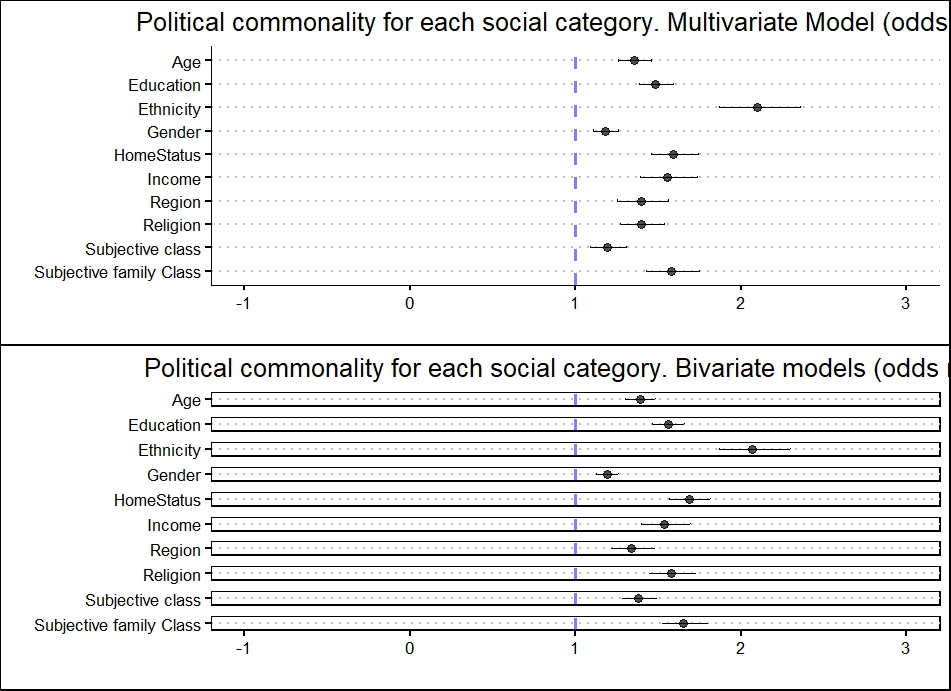
\includegraphics[width=1.3\textwidth]{Figure 2.jpeg}
    \caption{Replicating figure from original study}
    \label{fig:enter-label}
\end{figure}

Next, Figure 3 from the original study is replicated.
\\

Again, the original code to replicate Figure 3 is longer and can be found in the attached R file. I provide a snippet below:
\begin{verbatim}
    P.Homophily.3<-ggplot(InteractionIdentity.tidyP2, aes(x=Name,
    y=exp(Coefficient), col=Party)) + 
  geom_errorbar(aes(ymin=exp(Coefficient-2*SE), 
  ymax=exp(Coefficient+2*SE)), width=.2, position = position_dodge(width 
  = 0.5)) +
  geom_point(shape=19, size=2, position = position_dodge(width = 0.5)) +
  geom_hline(yintercept=1, linetype="dashed", 
             size=1, color="grey", alpha=0.5)+
  theme_clean()+ 
  ggtitle("Political commonality for each social category by party vote 
  in 2017 (odds ratio)") +
  labs(color = "General Election") +
  theme(plot.title = element_text(hjust = 0.5, face = "plain")) +
  xlab("") + ylab("")+
  coord_flip(ylim = c(0, 4))+
  facet_grid(Name~., scales="free", space = "free")+
  theme(strip.text.y = element_blank())+
  scale_color_manual(values= c("#0087DC", "#E4003B"), guide = 
  guide_legend(reverse=TRUE))

grid.arrange(P.Homophily.3, P.Homophily.4, nrow=2) 

\end{verbatim}



\begin{figure} [H] 
    \centering
    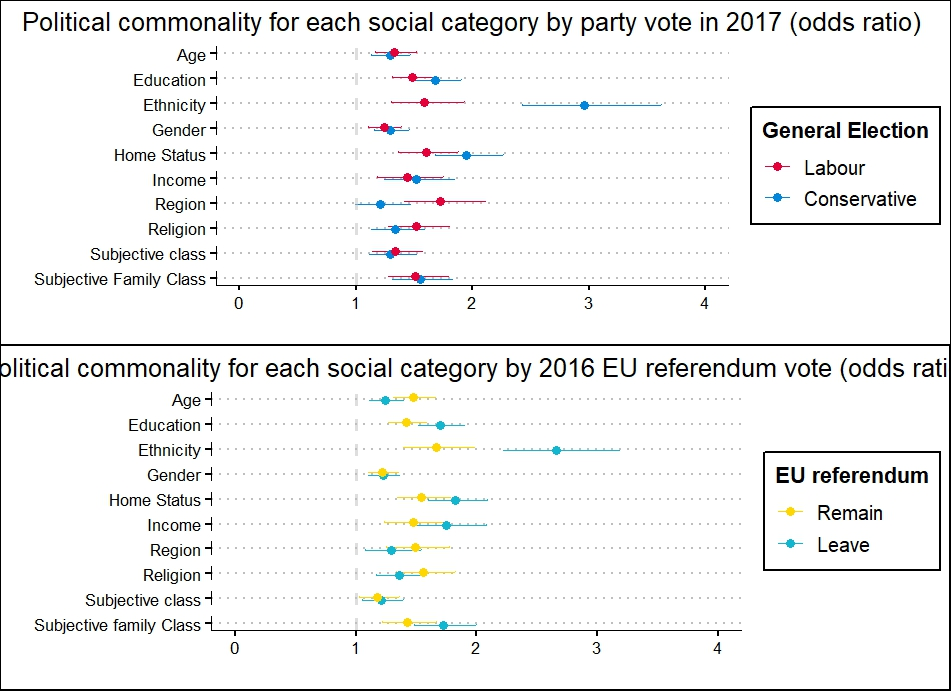
\includegraphics[width=1.3\textwidth]{Figure 3.jpeg}
    \caption{Replicating Figure from original study}
    \label{fig:enter-label}
\end{figure}


According to the author, "The relationship between perceived political commonality and vote choice is analysed by including the corresponding interaction effects in the regression model....Specifically, compared to Labour and Remain voters, Conservative and Leave voters give significantly more weight to ethnicity for perceived
political commonality"

\section{My Contribution}
The original study has an ordinal scale and the reference category is set 
to -1 which makes the findings hard to interpret substantively.
\\
\\
Hence, I relevel the outcome variables to a dummy variable (0 and 1) and 
run 2 separate logistic regression models:
\\
There are existing variables in the dataset which note whether a characteristic matches the respondent in Profile A/B. 
Model 1:
\\
Outcome variable:
\\
Respondents's choice, coded as:
\\
Respondent chooses Profile A = 1
\\
Respondent does not choose Profile A = 0
\\
\\
Input variable:
\\
Respondent's (Characteristic) is the same in Profile A = 1
\\
Respondent's (Characteristic) does not match Profile A = 0
\\
\\
Model 2
\\
Outcome variable: 
Respondent's choice coded as:
\\
Respondent chooses Profile B = 1
\\
Respondent does not choose Profile B = 0
\\
\\
Input variable:
\\
Respondent's (Characteristic) is the same as in Profile B = 1
\\
Respondent's (Characteristic) differs from Profile B = 0
\\
In order to do this, I relevel the outcome variables:
\begin{verbatim}
    data.experiment2.Second$ChoiceNFactorA <- 
    ifelse(data.experiment2.Second$ChoiceNFactor %in% c(-1, 0), 0,
    ifelse(data.experiment2.Second$ChoiceNFactor == 1, 1, NA))

    data.experiment2.Second$ChoiceNFactorB <- 
    ifelse(data.experiment2.Second$ChoiceNFactor == -1, 
    1,ifelse(data.experiment2.Second$ChoiceNFactor %in% c(0, 1), 0, NA))

\end{verbatim}

I run the first model:
\begin{verbatim}
    ProfileA <- glm(ChoiceNFactorA ~Match.GenderA 
    +Match.EducationA+Match.subClassA+
                  Match.subFamClassA+Match.HomeStatusA+
                  Match_regionA+  
                  Match_religionA+Match_ethnicityA+
                  Match_incomeA+AgeClosenessA
                , weights=data.experiment2.Second$W8,
                family = binomial(link = "logit"),
                data = data.experiment2.Second)

\end{verbatim}
This model explains the odds of a respondent picking Profile A if the respondent’s [characteristic] matches the characteristic in the profile
Below are the results of this model:

\begin{table}[H] \centering 
  \caption{Profile A Model (Odds Ratio)} 
  \label{} 
\begin{tabular}{@{\extracolsep{5pt}}lc} 
\\[-1.8ex]\hline 
\hline \\[-1.8ex] 
 & \multicolumn{1}{c}{\textit{Dependent variable:}} \\ 
\cline{2-2} 
\\[-1.8ex] & ChoiceNFactorA \\ 
\hline \\[-1.8ex] 
 Match.GenderA & 1.29$^{***}$ \\ 
  & \\ 
 Match.EducationA & 1.53$^{***}$ \\ 
  & \\ 
 Match.subClassA & 1.58$^{***}$ \\ 
  & \\ 
 Match.subFamClassA & 1.47$^{***}$ \\ 
  & \\ 
 Match.HomeStatusA & 1.35$^{***}$ \\ 
  & \\ 
 Match\_regionA & 1.42$^{***}$ \\ 
  & \\ 
 Match\_religionA & 1.54$^{***}$ \\ 
  & \\ 
 Match\_ethnicityA & 1.86$^{***}$ \\ 
  & \\ 
 Match\_incomeA & 1.67$^{***}$ \\ 
  & \\ 
 AgeClosenessA & 1.42$^{***}$ \\
  & \\ 
 Constant & 0.09$^{***}$ \\ 
  & \\ 
\hline \\[-1.8ex] 
Observations & 7,551 \\ 
Log Likelihood & $-$4,949.637 \\ 
Akaike Inf. Crit. & 9,921.275 \\ 
\hline 
\hline \\[-1.8ex] 
\textit{Note:}  & \multicolumn{1}{r}{$^{*}$p$<$0.1; $^{**}$p$<$0.05; $^{***}$p$<$0.01} \\ 
\end{tabular} 
\end{table} 
The interpretation for such a model is more intuitive in comparison to the original model:
When the respondent’s ethnicity matches the one in Profile A, the odds of the respondent selecting Profile A increase by a multiplicative factor of 1.86 on average, while holding all other variables constant


I do the same with Profile B:
\begin{verbatim}
    ProfileB <- glm(ChoiceNFactorB ~Match.GenderB 
    +Match.EducationB+Match.subClassB+
                  Match.subFamClassB+Match.HomeStatusB+
                  Match_regionB+  
                  Match_religionB+Match_ethnicityB+
                  Match_incomeB+AgeClosenessB
                , weights=data.experiment2.Second$W8,
                family = binomial(link = "logit"),
                data = data.experiment2.Second)


summary(ProfileB)

\end{verbatim}

\begin{table}[H] \centering 
  \caption{Profile B Model (Odds Ratio)} 
  \label{} 
\begin{tabular}{@{\extracolsep{5pt}}lc} 
\\[-1.8ex]\hline 
\hline \\[-1.8ex] 
 & \multicolumn{1}{c}{\textit{Dependent variable:}} \\ 
\cline{2-2} 
\\[-1.8ex] & ChoiceNFactorB \\ 
\hline \\[-1.8ex] 
 Match.GenderB & 1.12$^{**}$ \\
  & \\ 
 Match.EducationB & 1.47$^{***}$ \\ 
  & \\ 
 Match.subClassB & 1.52$^{***}$ \\
  & \\ 
 Match.subFamClassB & 1.09 \\ 
  & \\ 
 Match.HomeStatusB & 1.33$^{***}$ \\ 
  & \\ 
 Match\_regionB & 1.43$^{***}$ \\ 
  & \\ 
 Match\_religionB & 1.37$^{***}$ \\
  & \\ 
 Match\_ethnicityB & 2.00$^{***}$ \\ 
  & \\ 
 Match\_incomeB &  NA\\ 
  &  \\ 
  & \\ 
 AgeClosenessB & 1.28$^{***}$ \\
  & \\ 
 Constant & 0.13$^{***}$ \\ 
  & \\ 
\hline \\[-1.8ex] 
Observations & 7,520 \\ 
Log Likelihood & $-$5,053.354 \\ 
Akaike Inf. Crit. & 10,126.710 \\ 
\hline 
\hline \\[-1.8ex] 
\textit{Note:}  & \multicolumn{1}{r}{$^{*}$p$<$0.1; $^{**}$p$<$0.05; $^{***}$p$<$0.01} \\ 
\end{tabular} 
\end{table} 
When comparing this model to the original model, the odds ratio values are generally similar. A big difference is that the coefficient for Family class is not significant anymore
\\
\\
This model also raises questions as the original dataset has no instances where the income of the respondent matches the income of Profile B 


\end{document}
